\documentclass[12pt,halfparskip]{scrartcl}

\newcommand{\dokumenttitel}{Design}
\usepackage{../bodesuri}


\begin{document}

\title{\dokumenttitel}
\titlehead{
	\centering
	
\includegraphics[width=0.5 \textwidth, clip, trim = 0 7cm 0 0]{design/externes_design/bodesuri_plakat}
	\vspace{2cm}
}
\author{Danilo~Couto, Philippe~Eberli, \\ Pascal~Hobus, Reto~Schüttel, Robin~Stocker}
\maketitle
\newpage

\pagenumbering{roman}

\tableofcontents
\thispagestyle{plain}
\newpage

\pagenumbering{arabic}

\markright{Bodesuri -- \dokumenttitel}


\section{Systemstruktur} % (fold)
\label{Systemstruktur}

\subsection{Architekturübersicht} % (fold)
\label{sub:architekturuebersicht}

Bodesuri ist über mehrere Rechner verteilt. Es gibt vier Clients und einen Server pro Spiel. Der Client und der Server sind getrennte Programme, welche aber eine gemeinsame Codebasis haben.

Die Grundbausteine der Kommunikation zwischen Client und Server sind Zug und Zuginformation. Der Server sendet dem Spieler, der am Zug ist, eine Zugaufforderung. Auf die antwortet der Spieler mit einem Zug, welcher den Spieler, die gezogene Karte und die Bewegung der Figuren enthält. Der Server verteilt dann diese Informationen als Zuginformation an alle Spieler, wie man in Abbildung~\vref{fig:client_server} sehen kann.

\begin{figure}[h]
	\centering
	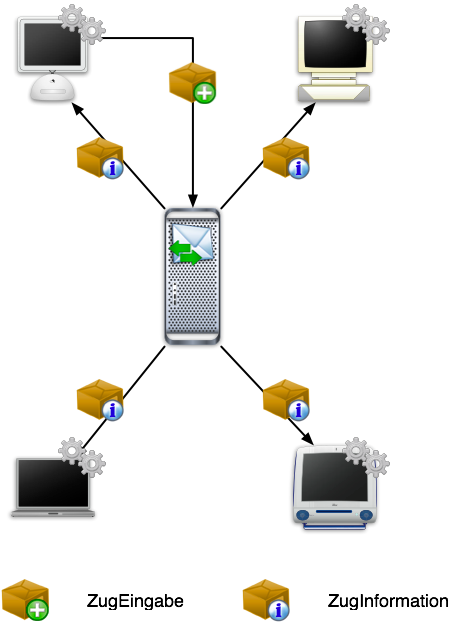
\includegraphics[width=0.7 \textwidth]{client_server}
	\caption{Kommunikation zwischen Client \& Server}
	\label{fig:client_server}
\end{figure}

Die Validierung der gespielten Züge geschieht beim Client, der Server ist zuständig für den Spielablauf.

\subsection{Architektonische Ziele \& Einschränkungen} % (fold)
\label{sub:architektonische_ziele_einschraenkungen}
\paragraph{Designentscheidungen}\label{ssub:designentscheidungen} % (fold)
\paragraph{Multitier Architektur des Servers}\label{ssub:multitier_architektur_des_servers} % (fold)
Der Server wurde in mehrere Schichten und vertikal angeordnete Partitions aufgeteilt. Diese Hierarchie hat sich deshalb als erforderlich erwiesen, da sonst Abhängigkeiten von tieferliegenden zu höherliegenden Schichten entstehen würden.
% paragraph multitier_architektur_des_servers (end)
\paragraph{Applikationsschicht}\label{ssub:applikationsschicht} % (fold)
Die Applikationsschicht wurde eingeführt, weil es wegen der Netzwerkfähigkeit viel Synchronisationsarbeit (z.\,B. für Zustände) gibt. Sie hat folgende Hauptaufgaben:
	\begin{itemize}
		\item Zustandssynchronisation als erste Vorstufe der Netzwerkkommunikation. Spezifische Nachrichten werden eingepackt, an die darunterliegenden Schichten weitergeleitet, um dann über das Netzwerk verteilt und empfangen zu werden.
		\item Controller-Komponente des MVC-Konzeptes, welche die Ereignisse im UI abfängt und verarbeitet, sowie Änderungen in der Problem Domain an das UI weiterleitet.
	\end{itemize}
% paragraph applikationsschicht (end)
% paragraph designentscheidungen (end)
\paragraph{Verwendete Entwicklungswerkzeuge}\label{ssub:verwendete_entwicklungswerkzeuge} % (fold)
Als Entwicklungswerkzeug wird MagicDraw UML verwendet. Es arbeitet Plattformunabhängig (Java), ist einfach handhabbar und hat sehr gute Funktionalitäten zur Code-Generierung. Die erzeugten Dateien lassen sich im XML-Format im SVN-Repository verwalten. Ein Nachteil ist, dass immer nur eine Person gleichzeitig an einem Projekt/Modul arbeiten kann, da MagicDraw UML keine SVN-Integration bietet und Konflikte nicht aufgelöst werden können.
% paragraph verwendete_entwicklungswerkzeuge (end)
\paragraph{Teamstruktur}\label{ssub:teamstruktur} % (fold)
Die Aufteilung des Teams ist aus den Arbeitspaketen in der Excel-Zeiterfassung ersichtlich. Die Verantwortlichkeiten sind in der Analysespezifikation geregelt.
% paragraph teamstruktur (end)
% subsection architektonische_ziele_einschraenkungen (end)

\clearpage
\section{Design Pakete} % (fold)
\label{design_pakete}

\subsection{Logische Sicht} % (fold)
\label{sub:logische_sicht}

Die logische Sicht beschreibt die Unterteilung der Architektur in die Schichten, Tiers, Packages und Klassen. Abbildung~\vref{fig:legende_diagramme} zeigt die Legende für die dafür verwendeten Klassendiagramme.

\begin{figure}[h]
	\centering
	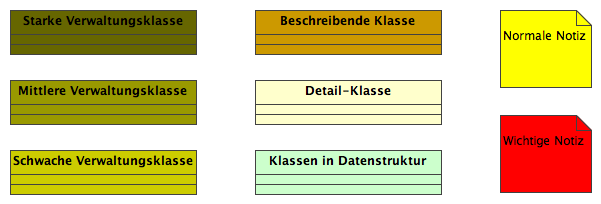
\includegraphics[width=\textwidth]{legende_diagramme}
	\caption{Legende der Diagrammfarben}
	\label{fig:legende_diagramme}
\end{figure}

\subsubsection{Schichtenarchitektur} % (fold)
\label{sub:schichtenarchitektur}
Für die logische Strukturierung des Projektes wird eine vierschichtige Architektur verwendet, wie in Abbildung~\vref{fig:architektur_schichten} dargestellt. Dabei setzt jede Schicht direkt auf den Diensten der darunterliegenden Schichten auf. Schichten können transparent sein. Dadurch ergeben sich wenige Indirektionen und eine einfache Nutzung der Dienste einer Schicht. Wo möglich und sinnvoll, werden Schnittstellen zwischen Schichten durch eine Fassade gebündelt, um die Kopplung zwischen den Schichten zu verringern. Dadurch lassen sich die Schnittstellen für die Schichten auch klarer definieren und sind einfacher zu nutzen. Im UI wird das MVC-Konzept verwendet, da eine komplexe Darstellungslogik durch das Spiel gegeben ist.
\begin{figure}
	\centering
	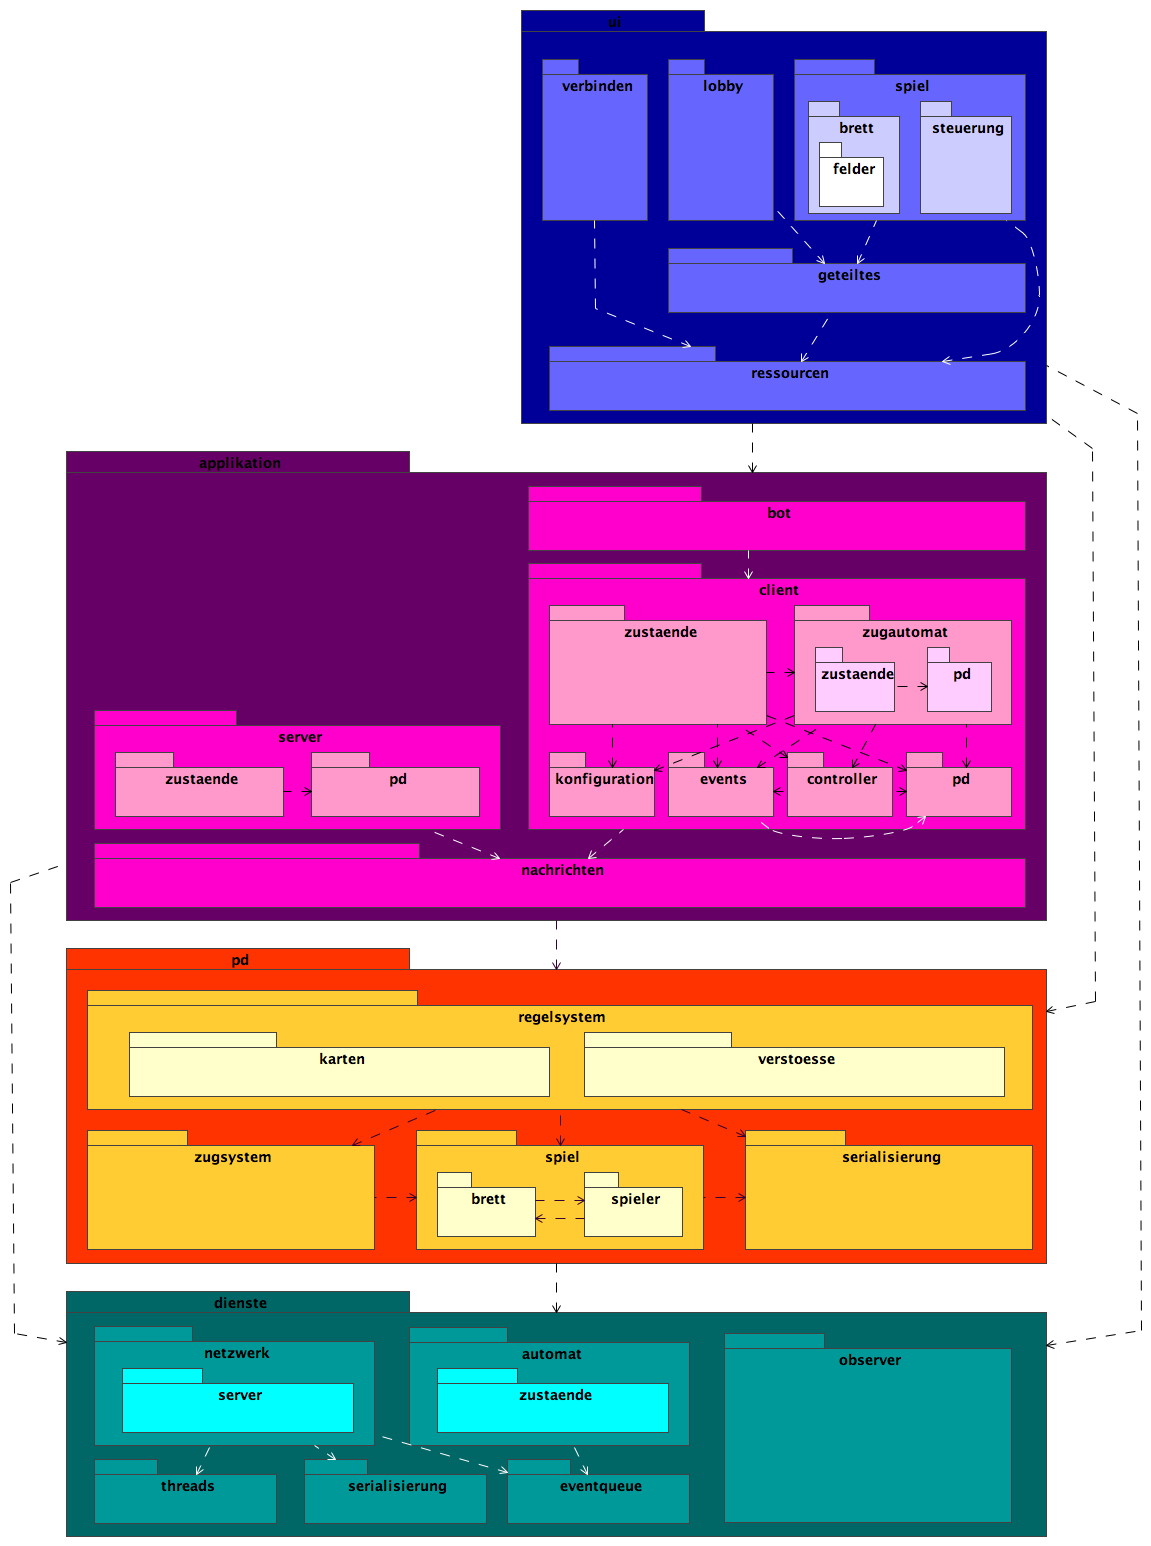
\includegraphics[width=\textwidth]{architektur_schichten}
	\caption{Schichtenarchitektur}
	\label{fig:architektur_schichten}
\end{figure}
% subsubsection schichtenarchitektur (end)

\clearpage

\subsubsection{Package pd} % (fold)
\label{ssub:package_pd}
\subparagraph{Beschreibung}
In der Problem-Domain-Schicht wird die gesamte Spiellogik gekapselt. Sie wird direkt von der darüberliegenden Applikationsschicht verwendet.

\subparagraph{Schnittstellen} % (fold)
\label{ssub:schnittstellen}
\begin{itemize}
	\item Package pd.zugsystem wird von applikation.zugentgegennahme verwendet, um Züge zu verarbeiten.
\end{itemize}
% subparagraph schnittstellen (end)
% subsubsection package_pd (end)

\clearpage
\subsubsection{Package pd.karten} % (fold)
\label{ssub:package_pd_karten}
\subparagraph{Beschreibung}
Beinhaltet alle Karten, die Kartenfarben, das Deck und den Kartengeber.

\subparagraph{Schnittstellen} % (fold)
\label{ssub:schnittstellen}
\begin{itemize}
	\item Als Einstiegspunkt für die Karten wird der Kartengeber verwendet, welcher das Mischen und das Ziehen einer Karte vom Stapel bereitstellt.
\end{itemize}
% subparagraph schnittstellen (end)

\begin{figure}[h]
	\centering
	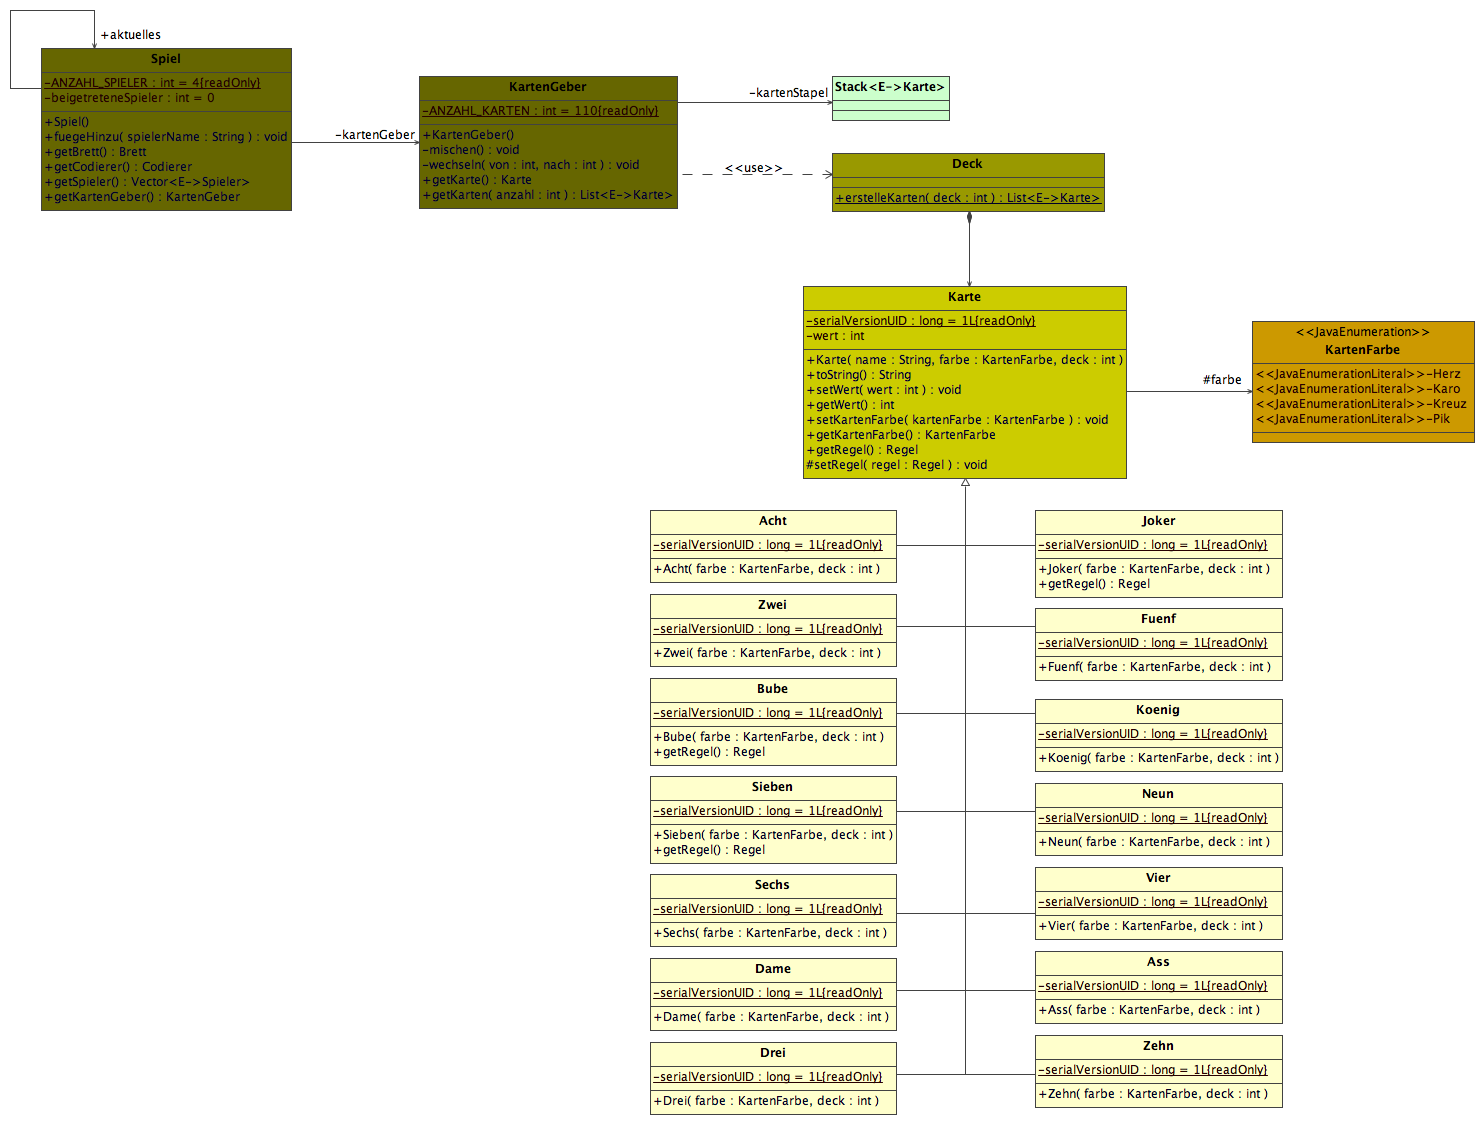
\includegraphics[width=\textwidth]{pd_kartengeber}
	\caption{Kartengeber}
	\label{fig:pd_kartengeber}
\end{figure}

% subsubsection package_pd_karten (end)

\clearpage
\subsubsection{Package pd.regelsystem, pd.zugsystem} % (fold)
\label{ssub:package_pd_regelsystem}
\subparagraph{Beschreibung}
Das Regel- und das Zugsystem sind eng miteinander verbunden. Sie nehmen die Aufgaben der Problem-Domain-Schicht wahr und stellen die Validierung der Züge sicher und berechnet die daraus resultierenden Aktionen in der Problem Domain (Figur von Feld X auf Feld Y verschieben).

\subparagraph{Schnittstellen} % (fold)
\label{ssub:schnittstellen}
\begin{itemize}
	\item Die Zugeingabe fasst die Informationen zusammen, die für einen Zug benötigt werden und über sie wird validiert, was zu einem ausführbaren Zug führt.
\end{itemize}
% subparagraph schnittstellen (end)

\begin{figure}[h]
	\centering
	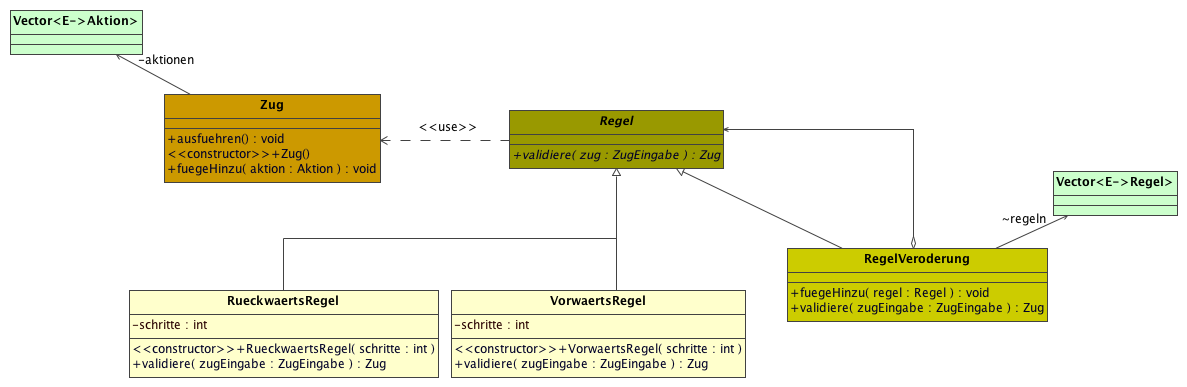
\includegraphics[width=\textwidth]{pd_regelsystem}
	\caption{Regelsystem}
	\label{fig:pd_regelsystem}
\end{figure}

% paragraph package_pd_regelsystem (end)

\clearpage
\subsubsection{Package pd.brett, pd.spieler} % (fold)
\label{ssub:package_pd_brett}
\subparagraph{Beschreibung}
Die beiden Packages sind eng miteinander verbunden und stellen die Abstraktion des Bretts (welches die Felder enthält), der Figuren und des Spielers in der Problem Domain dar.

\subparagraph{Schnittstellen} % (fold)
\label{ssub:schnittstellen}
Beschreibung der Schnittstellen
% subparagraph schnittstellen (end)

\label{ssub:diagramme}
\begin{figure}[h]
	\centering
	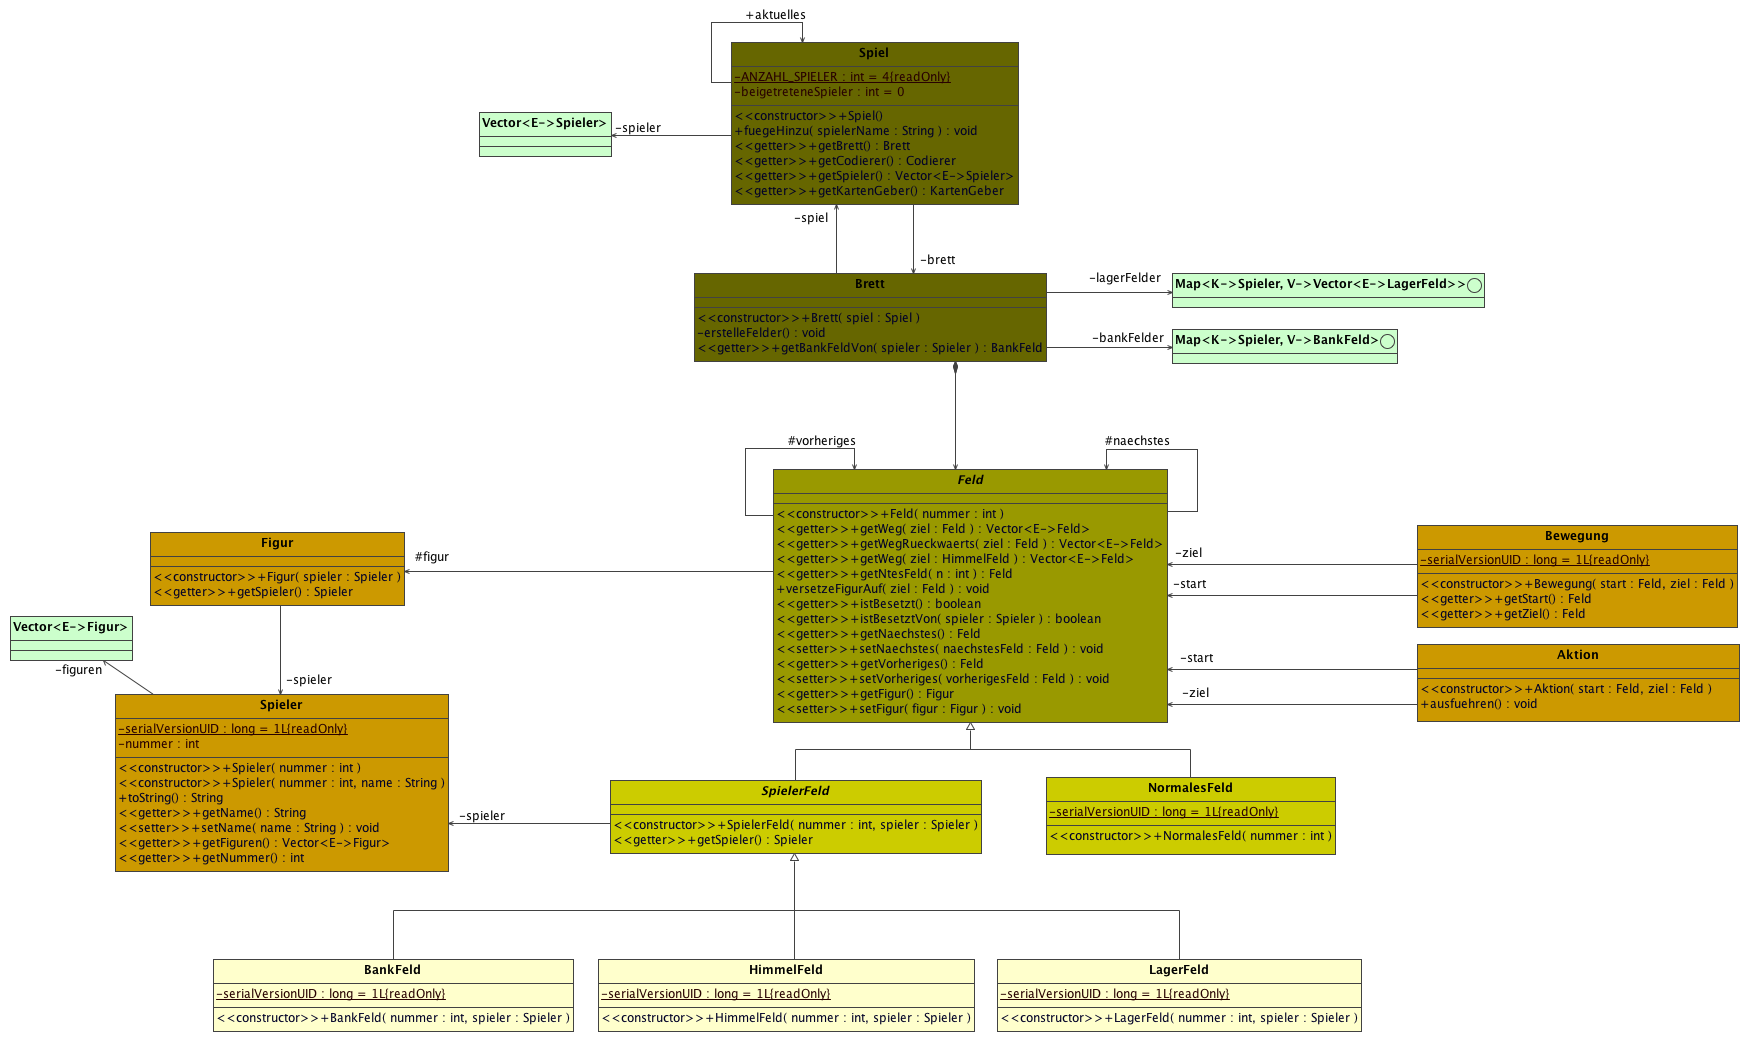
\includegraphics[width=\textwidth]{pd_brett}
	\caption{Brett und Figuren}
	\label{fig:pd_brett}
\end{figure}

% paragraph package_pd_brett (end)

\clearpage
\subsubsection{Package pd.serialisierung}

\subparagraph{Beschreibung}
Implementiert die abstrakten Klassen von dienste.serialisierung, um die Serialisierung von Klassen der Problem Domain zu ermöglichen.

\subparagraph{Schnittstellen}
\begin{itemize}
	\item Bietet eine Basisklasse (BodesuriCodierbaresObjekt) für die Klassen der Problem Domain an, die serialisiert werden können.
\end{itemize}

\clearpage
\subsubsection{Package pd.zustandsynchronisation} % (fold)
\label{ssub:package_pd_zustandsynchronisation}
\subparagraph{Beschreibung}
Beschreibung des Package. Aufgabe, etc…

\subparagraph{Schnittstellen} % (fold)
\label{ssub:schnittstellen}
Beschreibung der Schnittstellen
% subparagraph schnittstellen (end)
% paragraph package_pd_zustandsynchronisation (end)

\clearpage
\subsubsection{Package dienste.automat} % (fold)
\label{ssub:package_dienste}
\subparagraph{Beschreibung}
Beinhaltet einen Zustandsautomaten der im Client und im Server eine gezielte Abarbeitung
des Spielablaufs sorgt. Der Automat wechselt aufgrund externer Events auf vorher definierten
Bahnen zwischen den Zuständen hin und her.

\subparagraph{Schnittstellen} % (fold)
\label{ssub:schnittstellen}
\begin{itemize}
	\item Der Automat muss von den darüberliegenden Klassen abgeleitet und spezifisch implementiert werden.
\end{itemize}	
% subparagraph schnittstellen (end)

\begin{figure}[h]
	\centering
	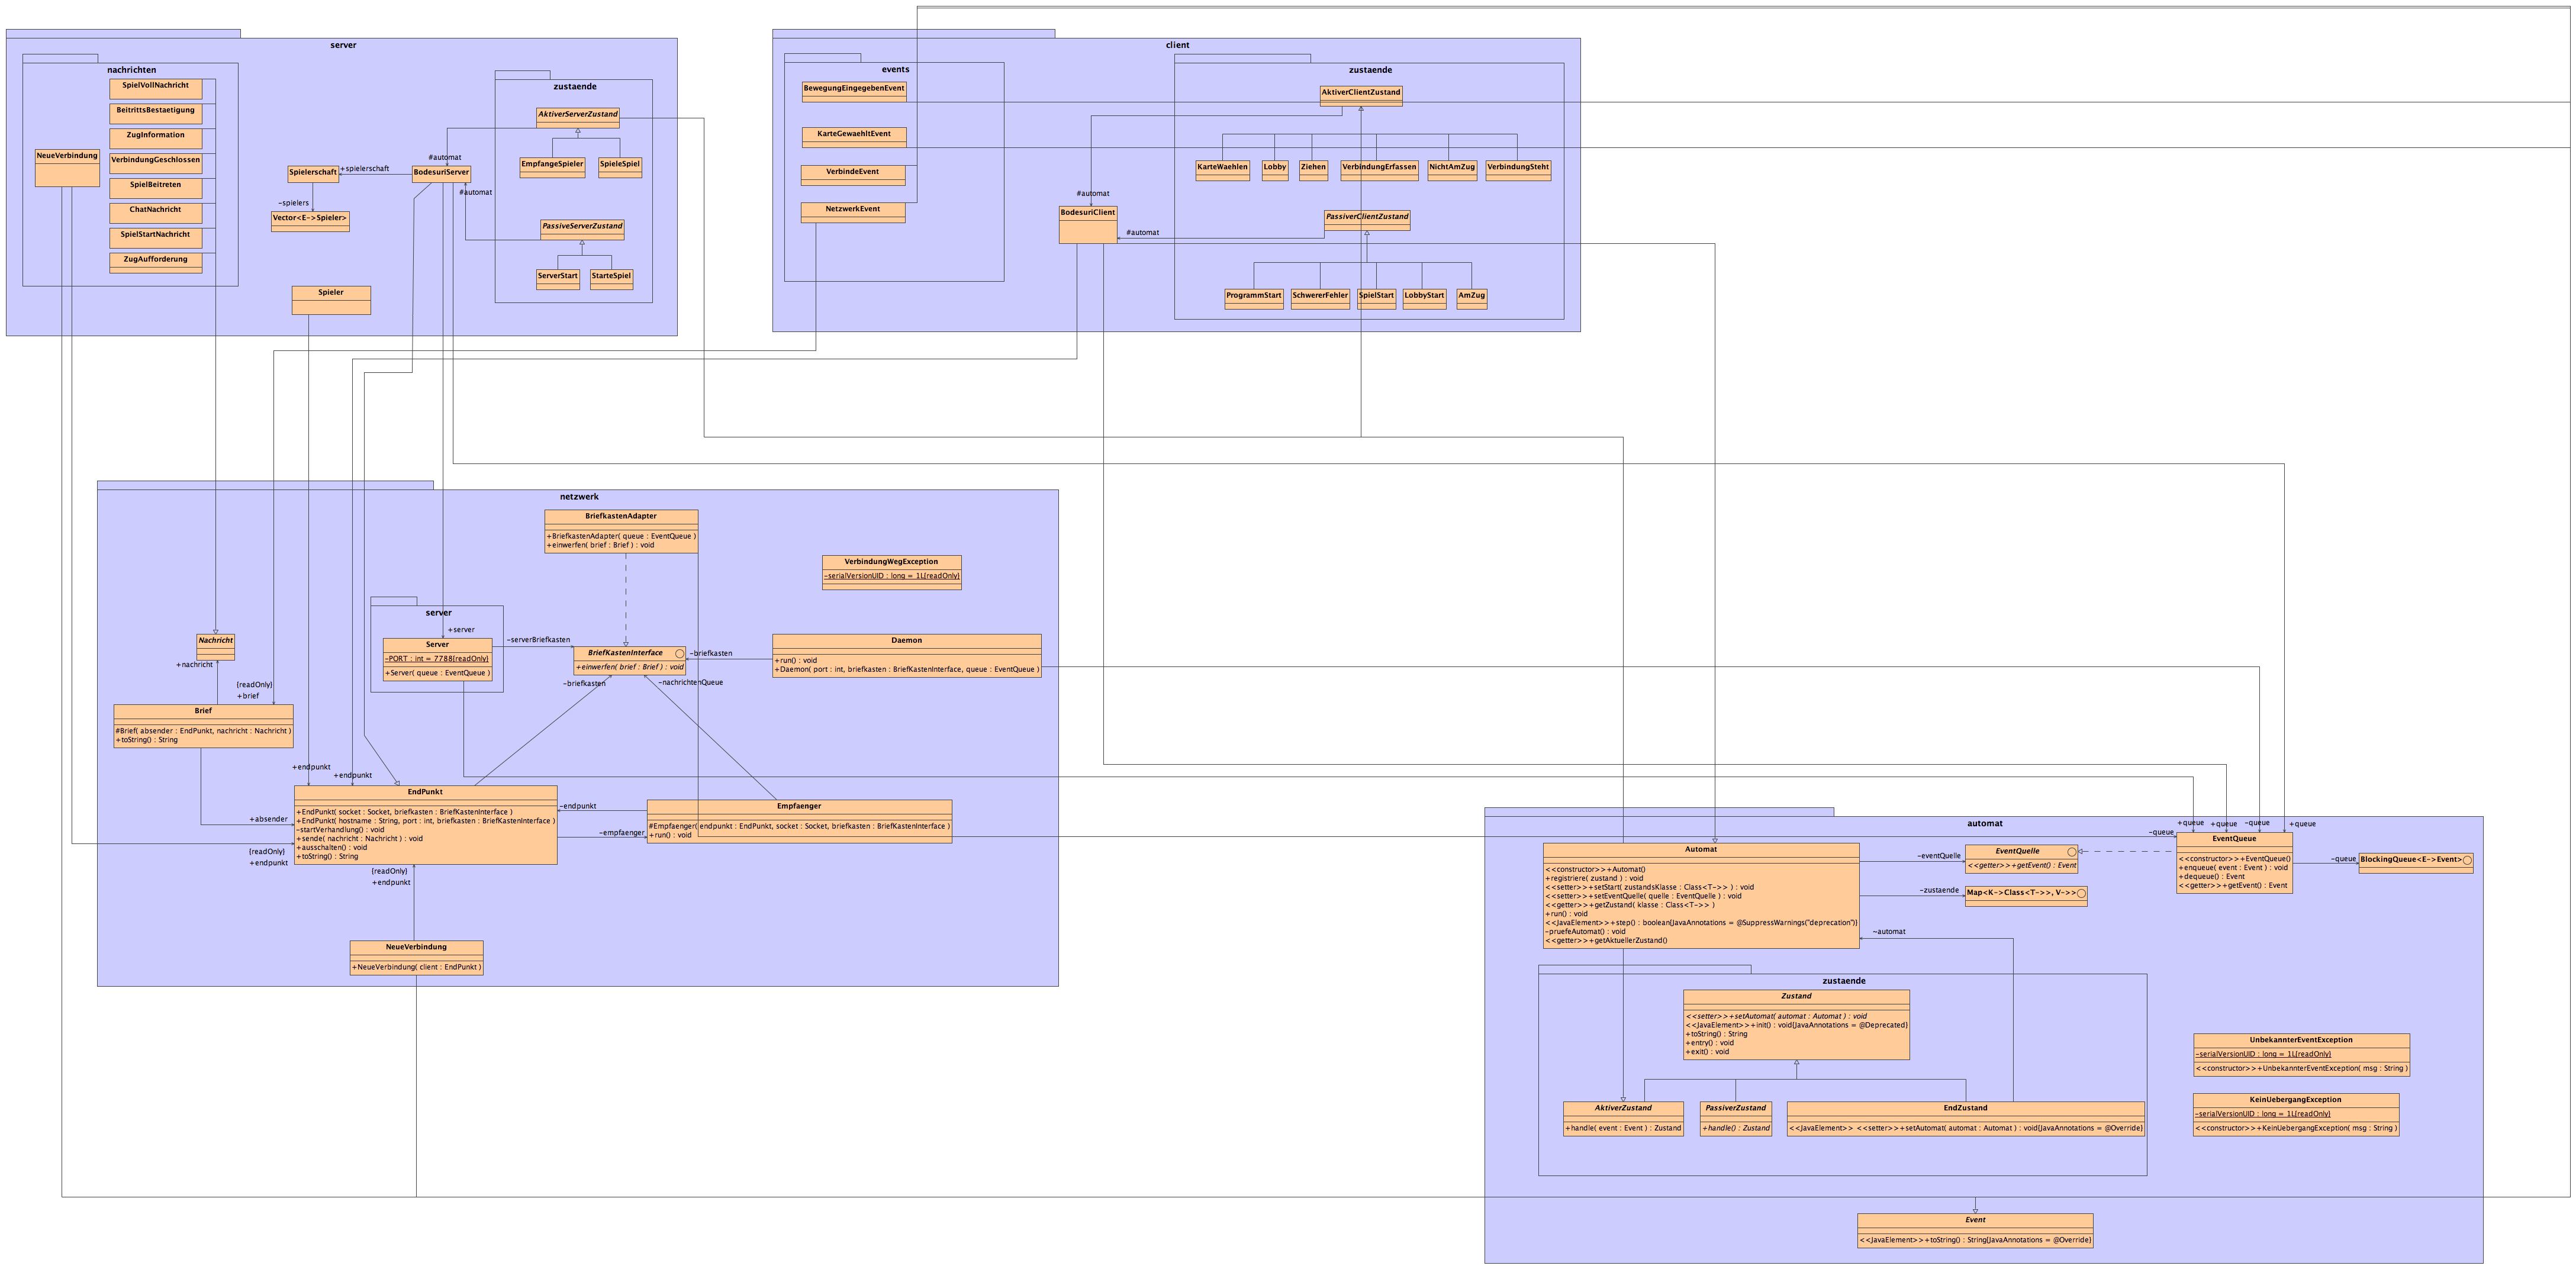
\includegraphics[width=\textwidth]{dienste_automat_klassendiagramm}
	\caption{Automat Klassendiagramm}
	\label{fig:dienste_serialisierung}
\end{figure}

% paragraph package_automat (end)

\clearpage
\subsubsection{Package dienste.serialisierung} % (fold)
\label{ssub:package_dienste_serialisierung}
\subparagraph{Beschreibung}
Dieses Package ist für die Serialisierung und Deserialisierung der Java-Objekte zuständig, welche anschliessend über das Netzwerk versendet werden.

\subparagraph{Schnittstellen} % (fold)
\label{ssub:schnittstellen}
Um die Serialisierung zu Nutzen, müssen die beiden abstrakten Klassen CodierbaresObjekt und CodiertesObjekt implementiert werden. In beiden muss die Methode getCodierer() implementiert werden, die eine Instanz des verwendeten Codierers zurückgibt. In CodierbaresObjekt muss zusätzlich noch die Methode getCodiertesObjekt(String code) implementiert werden, die ein neues konkretes CodiertesObjekt (z.\,B. BodesuriCodiertesObjekt) erstellen sollte.
% subparagraph schnittstellen (end)
% paragraph package_dienste_serialisierung (end)

\clearpage
\subsubsection{Package dienste.netzwerk} % (fold)
\label{ssub:package_dienste_netzwerk}
\subparagraph{Beschreibung}
Dieses Package kapselt die Socket-Schnittstelle von Java und bietet Dienste für die Netzwerkkommunikation an.

\subparagraph{Schnittstellen} % (fold)
\label{ssub:schnittstellen}
\begin{itemize}
	\item dienste.netzwerk verwendet die Klassen Event und EventQueue für die Kommunikation mit den darüberliegenden Schichten.
	\item Die Kommunikation mit dem Netzewrk findet über die Bibliotheken java.net statt.
\end{itemize}
% subparagraph schnittstellen (end)
% paragraph package_dienste_netzwerk (end)

\clearpage
\subsubsection{Package ui} % (fold)
\label{ssub:package_ui}
\subparagraph{Beschreibung}
Die UI-Schicht ist für die graphische Darstellung verantwortlich. Sie kommuniziert mit der Applikationsschicht top-down über direkte Assoziationen und bottom-up über Observer.

\subparagraph{Schnittstellen} % (fold)
\label{ssub:schnittstellen}
Beschreibung der Schnittstellen
% subparagraph schnittstellen (end)
% paragraph package_ui (end)

\clearpage
\subsubsection{Package ui.brett} % (fold)
\label{ssub:package_ui_brett}
\subparagraph{Beschreibung}
Beschreibung des Package. Aufgabe, etc…

\subparagraph{Schnittstellen} % (fold)
\label{ssub:schnittstellen}
Beschreibung der Schnittstellen
% subparagraph schnittstellen (end)
% paragraph package_ui_brett (end)

\clearpage
\subsubsection{Package ui.eigenschaften} % (fold)
\label{ssub:package_ui_eigenschaften}
\subparagraph{Beschreibung}
Beschreibung des Package. Aufgabe, etc…

\subparagraph{Schnittstellen} % (fold)
\label{ssub:schnittstellen}
Beschreibung der Schnittstellen
% subparagraph schnittstellen (end)
% paragraph package_ui_eigenschaften (end)

\clearpage
\subsubsection{Package ui.info} % (fold)
\label{ssub:package_ui_info}
\subparagraph{Beschreibung}
Beschreibung des Package. Aufgabe, etc…

\subparagraph{Schnittstellen} % (fold)
\label{ssub:schnittstellen}
Beschreibung der Schnittstellen
% subparagraph schnittstellen (end)
% paragraph package_ui_info (end)

\clearpage
\subsubsection{Package ui.ressourcen} % (fold)
\label{ssub:package_ui_ressourcen}
\subparagraph{Beschreibung}
Beschreibung des Package. Aufgabe, etc…

\subparagraph{Schnittstellen} % (fold)
\label{ssub:schnittstellen}
Beschreibung der Schnittstellen
% subparagraph schnittstellen (end)
% paragraph package_ui_ressourcen (end)

\clearpage
\subsubsection{Package applikation} % (fold)
\label{ssub:package_applikation}
\subparagraph{Beschreibung}
Die Applikationsschicht ist für die Zustandsynchronisation (Spielstände usw.) verantwortlich. 

\subparagraph{Schnittstellen} % (fold)
\label{ssub:schnittstellen}
Beschreibung der Schnittstellen
% subparagraph schnittstellen (end)
% paragraph package_applikation (end)

\clearpage
\subsubsection{Package applikation.zugentgegennahme} % (fold)
\label{ssub:package_applikation_zugentgegennahme}
\subparagraph{Beschreibung}
Beschreibung des Package. Aufgabe, etc…

\subparagraph{Schnittstellen} % (fold)
\label{ssub:schnittstellen}
Beschreibung der Schnittstellen
% subparagraph schnittstellen (end)
% paragraph package_applikation_zugentgegennahme (end)

\clearpage
\subsubsection{Package applikation.zustandsynchronisation} % (fold)
\label{ssub:package_app_zustandsynchronisation}
\subparagraph{Beschreibung}
Beschreibung des Package. Aufgabe, etc…

\subparagraph{Schnittstellen} % (fold)
\label{ssub:schnittstellen}
Beschreibung der Schnittstellen
% subparagraph schnittstellen (end)
% paragraph package_app_zustandsynchronisation (end)

% subsubsection design_pakete (end)
% subsection logische_architektur (end)

\clearpage
\subsection{Physikalische Sicht}

\subsubsection{Prozesse \& Threads} % (fold)
\label{sub:prozesse_threads}
Beschrieben, wie diese ablaufen, miteinander funktionieren, Daten austauschen, sich synchronisieren, etc...
% subsection prozesse_threads (end)


\clearpage
\section{Spielzustände \& Nachrichten} % (fold)
\label{spielzustaende_nachrichten}

\clearpage
\section{Dynamische Abläufe} % (fold)
\label{dynamische_ablauefe}

\begin{figure}[h]
	\centering
	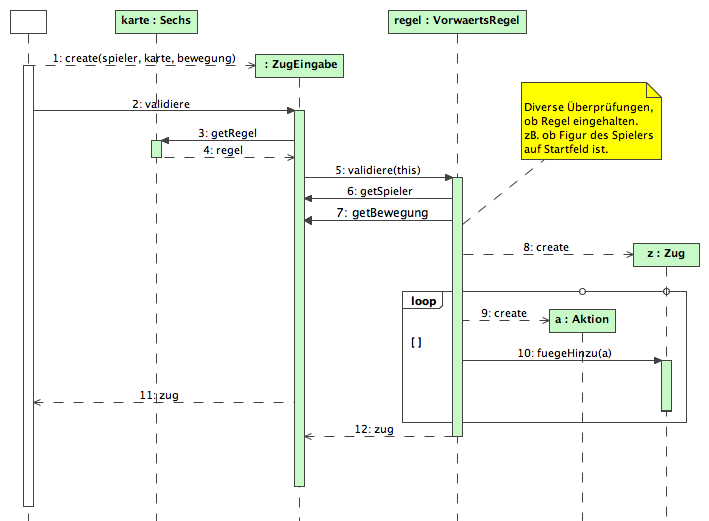
\includegraphics[width=\textwidth]{pd_validierung}
	\caption{Validierung von Spielzügen}
	\label{fig:pd_validierung}
\end{figure}

\begin{figure}[h]
	\centering
	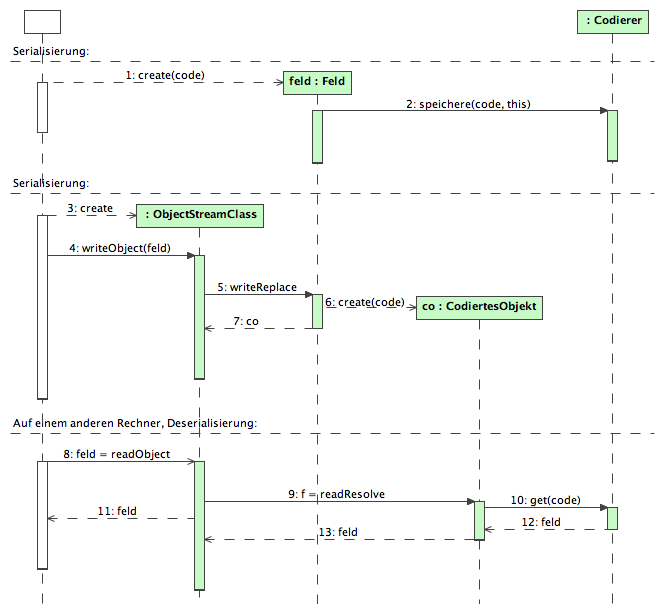
\includegraphics[width=\textwidth]{dienste_serialisierung}
	\caption{Serialisierung}
	\label{fig:dienste_serialisierung}
\end{figure}

\begin{figure}[h]
	\centering
	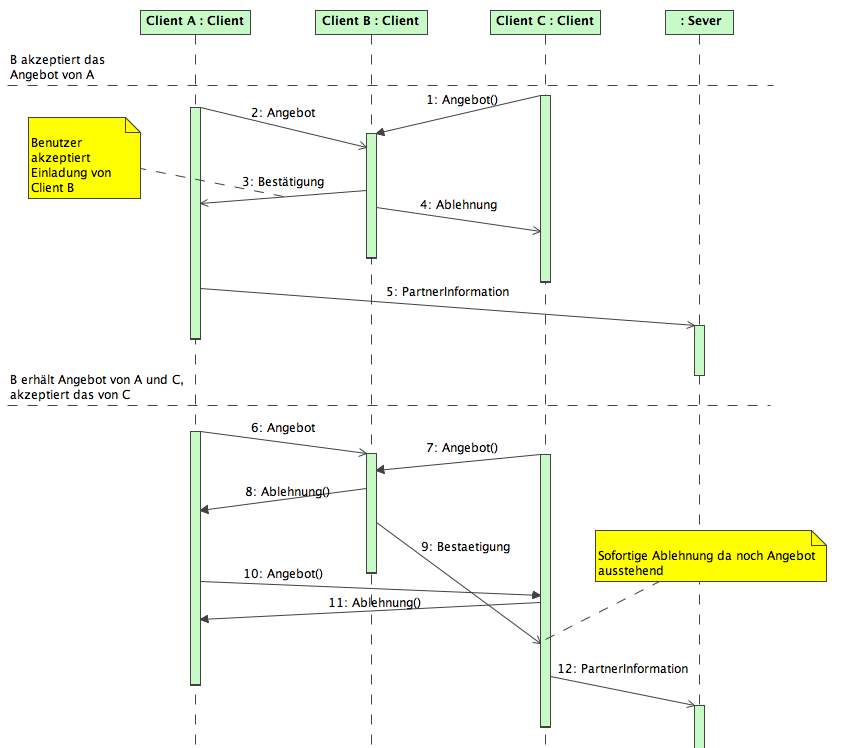
\includegraphics[width=\textwidth]{dienste_partnerschaft_normal_1}
	\caption{Normale Partnerschaft - Teil 1 von 2}
	\label{fig:dienste_partnerschaft_normal_1}
\end{figure}

\begin{figure}[h]
	\centering
	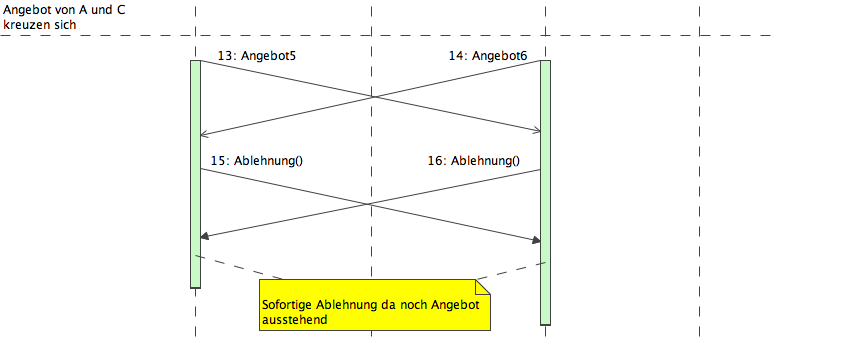
\includegraphics[width=\textwidth]{dienste_partnerschaft_normal_2}
	\caption{Normale Partnerschaft - Teil 2 von 2}
	\label{fig:dienste_partnerschaft_normal_2}
\end{figure}

\begin{figure}[h]
	\centering
	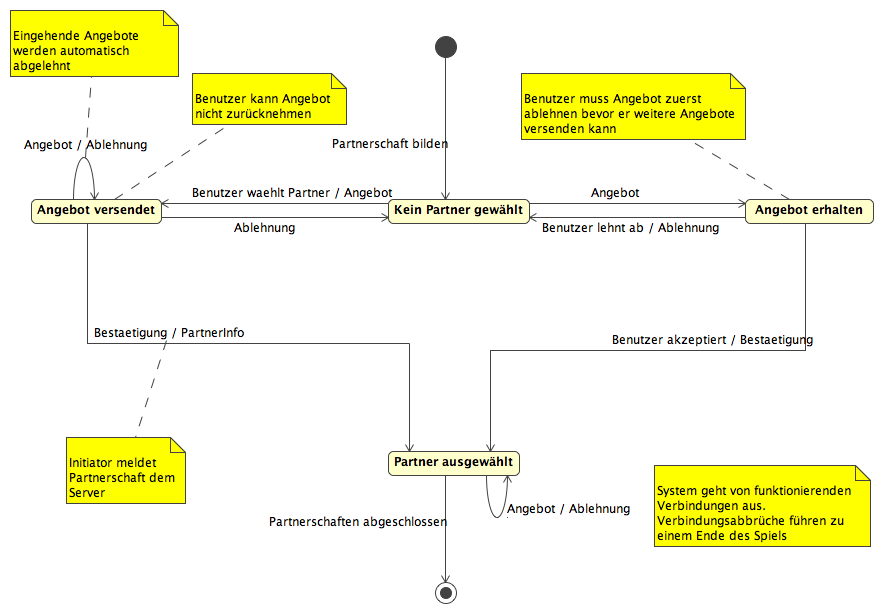
\includegraphics[width=\textwidth]{dienste_partner}
	\caption{Partner Verhalten}
	\label{fig:dienste_partner}
\end{figure}

\begin{figure}[h]
	\centering
	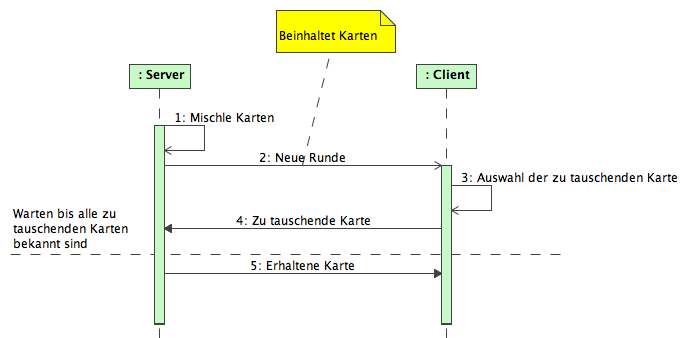
\includegraphics[width=\textwidth]{dienste_rundenstart}
	\caption{Rundenstart}
	\label{fig:dienste_rundenstart}
\end{figure}

\begin{figure}[h]
	\centering
	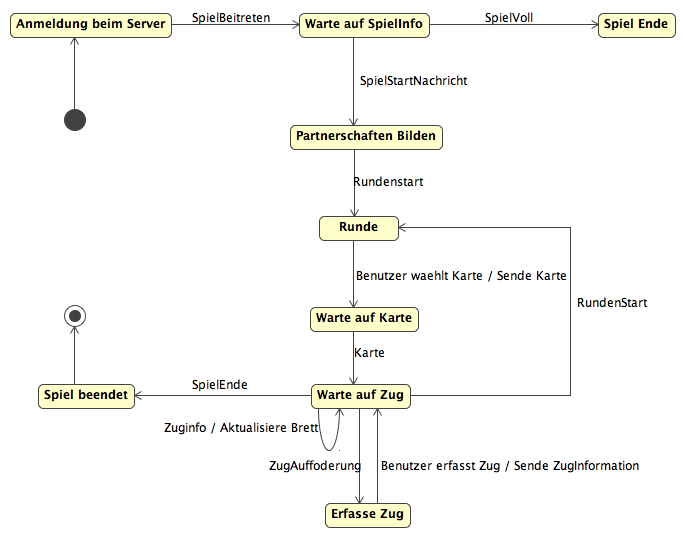
\includegraphics[width=0.8 \textwidth]{dienste_client}
	\caption{Zustände des Client}
	\label{fig:dienste_client}
\end{figure}

\begin{figure}[h]
	\centering
	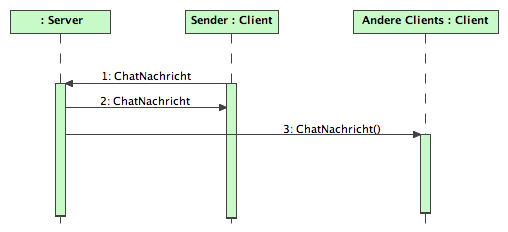
\includegraphics[width=\textwidth]{dienste_chat}
	\caption{Chat Subsystem}
	\label{fig:dienste_chat}
\end{figure}

\clearpage
\section{Externes Design} % (fold)
\label{externes_design}

\subsection{Verbindung zum Server} % (fold)
\label{externes_design_verbindung}

Beim Starten des Spiels wird der Spieler aufgefordert, die Serverdaten zur Verbindung eizugeben, sowie seinen Spielernamen.

\begin{figure}[h]
	\centering
	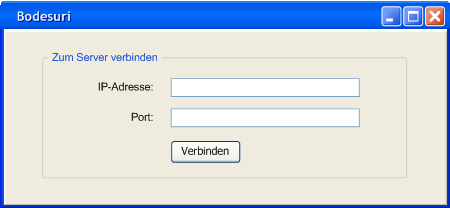
\includegraphics[width=0.7 \textwidth]{gui_verbindung}
	\caption{Verbindung zum Server}
	\label{fig:gui_verbindung}
\end{figure}

\clearpage

\subsection{Lobby} % (fold)
\label{externes_design_lobby}

In der Lobby können die Spieler einen Partner für das Spiel auswählen. Man wählt den Partner aus und gibt einen Gruppennamen ein. Nun muss nur noch der ausgewählte Partner die Anfrage akzeptieren, um die Gruppe zu bilden. Sobald der Spieler bereit ist, dem Spiel beizutreten wählt er im Spielstatus das Häkchen "<bereit"> aus. In der Zwischenzeit können sich die Spieler im Chat unterhalten (Priorität 3).

\begin{figure}[h]
	\centering
	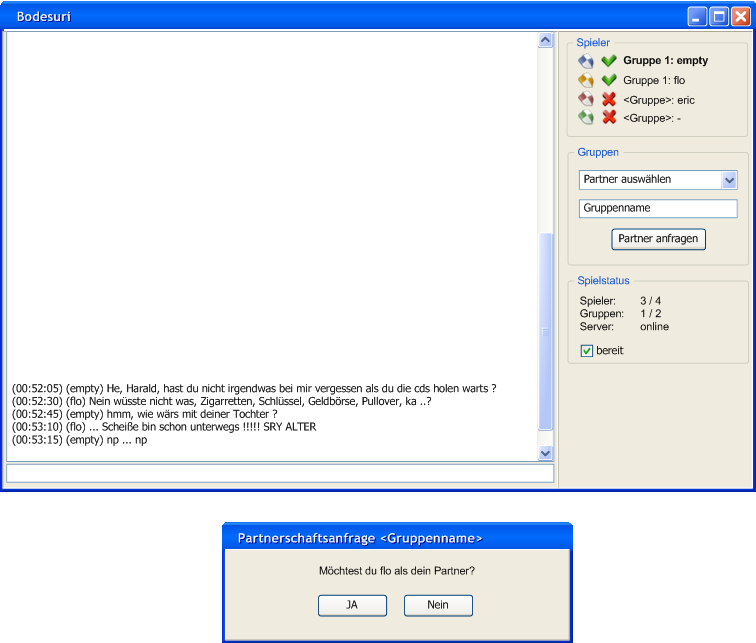
\includegraphics[width=0.9 \textwidth]{gui_lobby}
	\caption{Lobby vor dem Spielbeginn}
	\label{fig:gui_lobby}
\end{figure}

\clearpage

\subsection{Spiel} % (fold)
\label{externes_design_spielbrett}

Das Spiel besteht aus verschiedenen Views. In der BrettView wird das Spielbrett mit den Feldern und Spielfiguren dargestellt. In der SpielerView werden die einzelnen Spieler mit Gruppenzugehörigkeit aufgelistet. Die KartenView beinhaltet die Karten des Spielers. In der ChatView können sich die Spieler unterhalten (Priorität 3).

\begin{figure}[h]
	\centering
	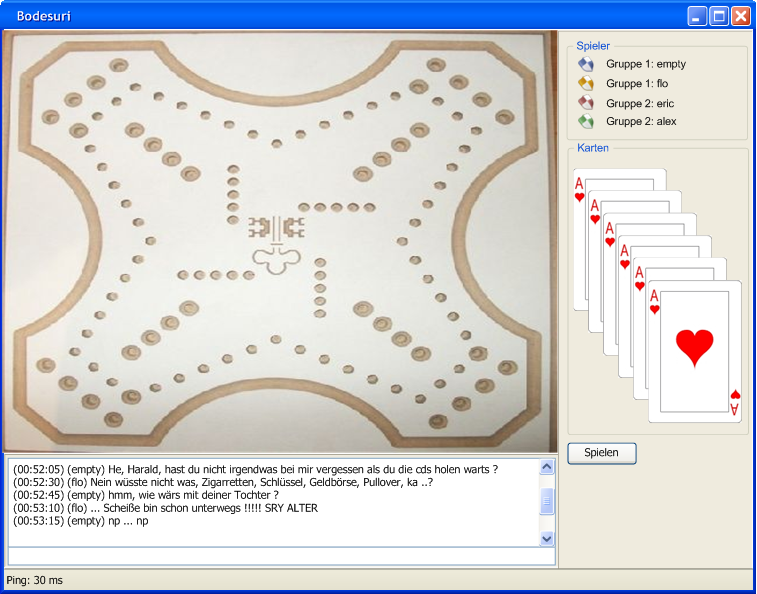
\includegraphics[width=0.9 \textwidth]{gui_spiel}
	\caption{Spielbrett}
	\label{fig:gui_spiel}
\end{figure}

% subsection externes_design (end)

\clearpage
\section{Eingetretene Risiken} % (fold)
\label{eingetretene_risiken}

\subsection{RMI} % (fold)
\label{sub:rmi}

Im Verlauf der ersten Tests mit RMI stellte sich schnell heraus, dass RMI weit mehr kann als für das Projekt notwendig wäre und es dem Projekt somit unnötig Komplexität hinzufügt. Andererseits stellt RMI  einige Anforderungen an die Client/Server-Struktur, die sich nur schwer mit den Projektanforderungen decken lassen. So kann RMI nur erschwert hinter Firewalls betrieben werden und eine Kommunikation über ein durch NAT\footnote{Network Adress Translation. Firewall-Feature welches Netzbereiche auf andere Netzbereiche abbildet. Wird häufig verwendet, um private Adressbereiche im Internet hinter einer einzelnen Adresse zu verstecken.} verstecktes Netzwerk ist gar nicht erst möglich. Da die Internet-Zugangslösungen in den meisten Haushalten auf Firewalls und NAT basieren, könnte das Spiel von einem grösseren Teil der potenziellen Kundschaft gar nicht gespielt werden.

Wir entschieden uns auf Grund dieser Probleme, auf eine eigene Lösung umzusteigen, welche auf den Java-Klassen Socket und Object(Input|Output)Stream basiert. Insgesamt gingen etwa 10 Stunden Arbeit für diese Umstellung verloren.
% subsection rmi (end)

\subsection{Java 2D} % (fold)
\label{java_2d}

Nachdem das CLI (Command Line Interface) erstellt war, entwarfen wir ein GUI dafür, das die Felder und Figuren darstellen sollte. Mit Java 2D ist das Zeichnen sehr einfach, da man die Koordinaten der zu zeichnenden Elemente angeben kann. Doch mussten wir leider feststellen, dass das Ansprechen eines Objektes etwas komplizierter ist. So muss zum Beispiel bei einem Mausklick das geklickte Objekt über die Koordinaten ermittelt werden. Ausserdem muss man sich um das Aktualisieren der Anzeige bei Veränderungen selber kümmern.

In einem zweiten Versuch erstellten wir das selbe Spielbrett mit Swing und wir kamen zum Schluss, dass dies die einfachere Methode ist. Die Objekte können mit einem speziellen Layout auch auf Koordinaten genau platziert werden und Klicke darauf kann man wie gewohnt mit einem MouseListener abfangen. Als Objekt kann man zum Beispiel ein Label mit einem Icon verwenden. Dies reicht für ein Brettspiel vollkommen aus.

Aus diesen Gründen haben wir uns dazu entschlossen, für das GUI als einzige Technologie Swing einzusetzen. Insgesamt gingen 7.5 Stunden Arbeit für diese Umstellung verloren.

% subsection java_2d (end)

% section eingetretene_risiken (end)

\end{document}
